\newpage
\chapter{Methodology}
In the following chapter, the component analysis is defined first. This results in the requirements that must be considered in the design when implementing the extension, which is then discussed in the third section. In the final section, the tests, to ensure that the extension matches the expected requirements and it is defect free, are described.

\section{Requirements Elicitation and Analysis}
The extension is used to improve the user's experience when navigating through an e-commerce website to search for a wanted product or service. The idea is to integrate the end user's browser with an extension, which will record the host name or domain of the visited website's URL along with the respective parameters. When enough records have been collected, the extension will display a list of parameters for the visited domain. Path parameters and query parameters will be separated from these parameters. The user can then navigate through the path parameters in the same way that they would navigate through a file system. When the last path parameter is reached, the query parameters and the number of times these parameters are called in the URL are displayed. Below the list is an input field and a button; these input fields will be filled based on and while navigating through the selected parameters. When the "Navigate" button is clicked, a new tab will open with the full-path built URL.

These prerequisites and considerations result in the following requirements for the extension, which is to be developed within the scope of this thesis. These requirements are classified into functional and non-functional requirements.

\subsection{Functional Requirements}
A requirement is called functional if its underlying need is functional, i.e., it relates to information processing objects (data, operations, behavior). In other words, functional requirements are statements of services the system should provide, how the system should react to particular inputs and how the system should behave in particular situations \autocite{sommerville2011software}. The following functional requirements are defined for the extension:

\begin{itemize}
  \item FR-01: User can see how many times each query parameters for each host name are used
  \item FR-02: User can build a URL query string based on their history
  \item FR-03: User can navigate to the URL with the built query string
\end{itemize}

In addition to functional requirements, non-functional requirements are also defined as follows.

\subsection{Non-Functional Requirements}
A requirement is called non-functional if its underlying need is a non-objective property. In other words non-functional requirementes are constraints on the services or functions offered by the system such as timing constraints, constraints on the development process, standards, etc \autocite{sommerville2011software}. It often apply to the system as a whole rather than individual features or services. The following non-functional requirements arise for the extension to be developed:

\begin{itemize}
  \item NFR-01: UI components must be implemented using React.
  \item NFR-02: TypeScript must be used to implement dynamic functions.
  \item NFR-02: Data must be saved on the end-user's Chrome storage.
  \item NFR-03: Both the external components used and the developed component itself must be well documented.
  \item NFR-04: The individual external libraries must be easy to update.
  \item NFR-05: Modularization must be taken into consideration throughout development so that individual modules and/or components can be easily reused, expanded or changed.
\end{itemize}

While functional requirements are perceived as such by the user, non-functional requirements are implementation details that remain largely hidden from the user.

\section{Design Concept}
The original concept of this thesis is to create an additional feature for marta's customer-facing platforms. Marta as a business is currently best described as a marketplace between caregivers and families requiring 24-hour care. 24-hour care can be defined as living in a household with the person in need of care for a certain period of time. This means that caregivers are primarily responsible for basic care and household chores. In addition, they support the person in care's relatives in need of assistance in carrying out the activities they wish to do. Marta as a marketplace connecting families with caregivers is competing against more traditional agencies, where it can take several days or even weeks to find a family for a newly signed up caregiver or the other way around.

As a growing start-up that gained a lot of users in the past few months, marta would need to enhance their product, to compete in this expeditiously developing business. One way marta can provide a superior experience for both caregivers and families is to speed up the matching process between both parties. The caregiver and family inquiry forms are designed to record as much information as possible which can be used during the matching phase. The matches are then created by the teams in Berlin and Romania. To make the job more seamless, the technical team in marta introduced a "matching score" by which possible matches are sorted. As a result, a number of caregiver profiles with high matching scores are shown to the family. Filter functionality is provided to speed up the search process. This includes caregiver's earliest starting date, German skills, experience with diseases, etc.

Marta needs to introduce a continually improved, user-friendly filtering functionality to adjust to the needs of their users. An example of a user-friendly filter would be to provide quick filter suggestions which the user can click once and the desired results will be shown, instead of letting users select the same filter manually over and over again. In order to determine which filter suggestions are the most beneficial, frequently used filters need to be identified.

A question arose within this world of thought about how to improve the existing filtering functionality for a better user experience. An early concept was to create quick filters within the application that suggested to users which filters they frequently used. For example, if a family is looking for a caregiver with German speaking capability level 3, the German filter would be activated. Each filter usage will be counted and saved to a relational database. The three most frequently used filters will be displayed as quick filters for all users, and the user will only need to click on those quick filters to activate them. Not only that, the user can also combine those quick filters to narrow the search even further.

The first problem with this idea was that it collected filter usage data from every user and stored it without providing any detailed information about who used the filter and when it was used. Each family's search criteria are unique. Hence the first idea would not be as beneficial to the users. We must also keep in mind that this approach will only benefit those who actively use the platform. The second concern was that if the filter recommendations were tailored to each individual user, the amount of data maintained would rapidly grow to be rather large. It would be a waste of storage space and would not be sustainable, especially if the number of filters and users grows. We would develop quick filters not only on one page, but on several. And each would require the same amount of storage space.

The concept was then expanded upon and a decision was reached. Instead of adding those quick filters directly into the platform, an extension that allows for even more personalized filter suggestions should be developed. The aforementioned issues can be addressed by developing an extension. The information that will be saved varies for each user and is saved in the end user's browser, which means that other users' activity will not impact the filter suggestions. Furthermore, search and filter is a popular website design method. It would benefit not just Marta's platform, but also other e-commerce websites like Lacoste, Nike, Adidas, and others. Moving it to an extension would allow people to choose whether or not to install it. And, because this is a separate capability with a different software architecture than Marta's primary platform, a new repository or codebase is developed to make it easier to distinguish and manage.

\section{Technologies}
\label{technologies_used}

%Browser Extension
\subsection{Browser Extension}
Browser extensions or addons are third party programs, that can extend the functionality of browsers and improve users' browsing experience \autocite{some2019empoweb}. A browser extension, as opposed to a standard web page, is created specifically for a given browser and uses that browser's extension API. It was necessary to choose a browser as a result. There are frameworks that try to make it feasible to create an extension for several different browsers at once. Although the caliber of these frameworks was unclear, it was decided that the expense of potential problems and additional time spent debugging in many browsers outweighed the benefits.

%Chrome Extension Architecture
\subsection{Chrome Extension Architecture}
Extensions are built on web technologies such as HTML, JavaScript, and CSS. They run in a separate, sandboxed execution environment and interact with the Chrome browser \autocite{google2021what}. They also have access to the APIs that browsers provide for tasks like XMLHttpRequests and HTML5 features on web sites. The following files can be found in an extension:

\begin{itemize}
  \item A manifest.json file
  \item One or more HTML files
  \item Any other files such as CSS or JavaScript needed by the extension to run
\end{itemize}

The majority of extensions have a background page that contains their primary logic and state. They frequently also contain content scripts that can communicate with websites. Asynchronous message passing is used to communicate between the background page and the content scripts. Additionally, extensions can save data via localStorage and other HTML5 storage APIs.

\subsection*{Manifest Files}
A manifest.json file is required for each extension. It includes crucial information about the extension, such its name, version, scripts used for its content, minimum Chrome version, and permissions. The content-scripts field was the most crucial one for this expansion. Each study and content-related webpage need its own content script. Each one was defined in the scripts column, which also mapped each one to the appropriate URLs.

\subsection*{Content Scripts}
Content scripts are JavaScript files that are used on websites to add new functionality. They have full control to modify the entire web page because they can directly access the DOM of these web sites. The content script is injected into a tab when the web page is loaded, and runs in the same process space of the renderer of the web tab and can thus access its DOM objects. Injected content scripts in a tab can only communicate with the extension core via Chrome's IPC \autocite{liu2012chrome}.

\subsection*{Service Worker}
The Chrome extension platform switches from background pages to service workers in Manifest V3. A service worker is a script that your browser runs in the background, distinct from a web page, opening the door to features that don't need a web page or user input \autocite{chrome2021service}. This technology allows native-like experiences over the open web, including push notifications, robust offline support, background synchronization, and "Add to Home Screen." Service providers drew some of their inspiration from the background pages in Chrome Extensions, but improvements were added for the web.

Service workers are specialized JavaScript assets that act as proxies between web browsers and web servers. They aim to improve reliability by providing offline access, as well as boost page performance \autocite{chrome2021service}. Websites are gradually improved by service workers through a lifetime akin to that of platform-specific programs.

\subsection{Choice of Implementation Browser}
The selection of a browser was based on a number of factors. The first was the browser's usage rate. This is significant since anyone who doesn't already have the necessary browser will need to download and install it. Drop-outs due to the installation process or being unfamiliar with a new browser can significantly raise the cost of conducting the survey. The ease of use of the API and simplicity of implementation were additional crucial criteria. The extension programming process should ideally only need a basic understanding of the extension API. The capabilities of the API offered by the browser was another factor considered. The extension needs to:

\begin{enumerate}
  \item Store a big amount of data on the client side
  \item Read URL - so path and query string can be passed to the extension
  \item Modify URL - so frequently used path and query string can be utilized
  \item Open a full-path URL in a new tab
  \item Access opened tabs
\end{enumerate}

After 25+ years of helping people use and experience the web, Internet Explorer (IE) is officially retired and out of support as of June 15, 2022. Thus, IE was eliminated from the list, leaving Firefox and Chromium-based browsers (such as Google Chrome, Microsoft Edge, Opera, Vivaldi) as the options.

Both the Firefox and Chrome extension APIs provided comparable functionality. To a considerable degree, Firefox's extension technology is compatible with the extension API used by Chromium-based browsers. Most extensions designed for Chromium-based browsers operate in Firefox with very minor modifications. One disadvantage was that Mozilla only support Manifest V2 and not V3. Since announcing Manifest V3 in 2018, Google has launched Manifest V3 in Chrome, started accepting Manifest V3 extensions in the Chrome Web Store, co-announced joining the W3C WebExtensions Community Group (formed in collaboration with Apple, Microsoft and Mozilla), and, most recently, laid out a timeline for Manifest V2 deprecation. New Manifest V2 extensions will no longer be accepted as of January 2022, and Manifest V2 will no longer function as of January 2023 \autocite{alexei2021manifest}. Manifest V3 dictates an ecosystem change that limits Manifest V2 extensions and would likely force Manifest V2 based extensions to conform to Manifest V3 in the near future.

\begin{figure}[ht!]
  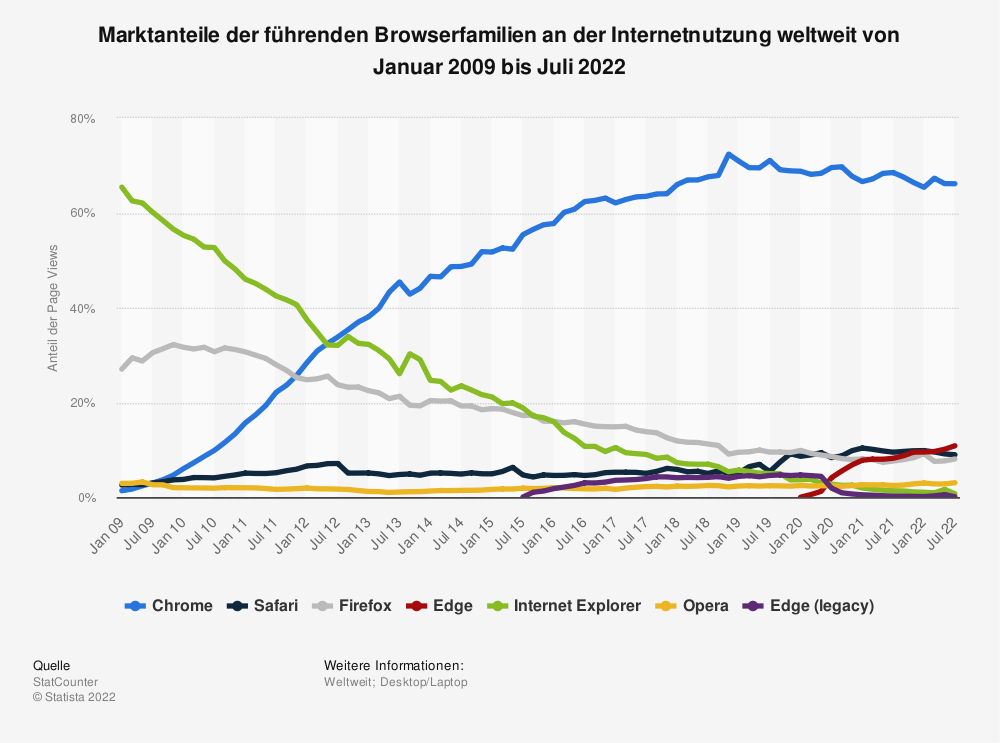
\includegraphics[width=\textwidth]{assets/statistic_id157944_marktanteile-fuehrender-browser-weltweit-bis-juli-2022.png}
  \caption{Market shares of leading browsers worldwide by July 2022}
  \label{fig:browserMarketShareChart}
\end{figure}

Additionally, it was discovered that the Chrome documentation was easy to grasp and was divided up into sections. Chrome also has an overwhelming market share: over two-thirds of all users globally use Chrome as their browser (See Figure ~\ref{fig:browserMarketShareChart}). As a result, it was decided to develop a Chrome-based browser extension.

%React
\subsection{React}
\label{react}
React is a product of Facebook's engineering team, which is a JavaScript framework for creating user interfaces \autocite{gackenheimer2015introducing}. Because of its simplicity and straightforward but efficient development process, React is quite well-liked in the developer communities. Interactive user interfaces are simpler to develop with React. It effectively updates by accurately drawing each state's view's constituent parts, and it updates the application's data \autocite{islam2017reactjs}. The core objective of React is to provide the best possible rendering performance. Its strength comes from the focus on individual components. Using reusable components, it is found to be easy development for developers to design rich UI's. React incorporates with View part from MVC model \autocite{maratkar2021re}. React implements One Way dataflow so that it gets easier than traditional data binding. React uses virtual DOM it offers not so complex programming with faster execution. It makes use of composition to create intricate user interfaces out of simple building blocks known as Components \autocite{david2020building}.

\subsection*{Component}
Each component has a render method, which can either return HTML or another React component, and returns a description of what to render. A combination of HTML and Javascript known as JSX is used to describe what should be rendered. A more detailed explanation of JSX is included in the JSX section. It is possible to specify a component as a class or a function. Props and state are crucial components when creating React applications.

\subsection*{States and props}
The state of a component allows it to "remember" things, and it can change in response to user interaction or other application-wide actions. The State is optional; components without a state are referred to as presentational components. Components with a state are referred to as stateful components.

Immutable data supplied into a component during development is known as props, or properties. Because a component can function and seem differently depending on the properties supplied into it, props enable React components to be flexible and reusable.

Using props, data moves down the component tree in React. Callback functions are supplied as props so that a child component can communicate with its parent. Callback methods and other data must be passed down numerous layers in large React apps due to the component tree's depth. Props-drilling is a technique that results in tightly connected components and a less maintainable program. This is one of the reasons why complex React apps require architectural patterns.

\subsection*{Class-based components}
A class-based Component is created by extending the React.Component class. The state of a class-based component is updated using the method setState() and read by using this.state within the class. Using the setState() method makes the component re-render which is not the case when mutating the state directly. Class-based components include life-cycle methods that can be used to create more complex behavior. It also requires a render method to return JSX elements.

\subsection*{Life-cycle methods}
Life-cycle methods are built-in functions that are called whenever a state or prop updates, a component renders, is destroyed, or both.

\subsection*{Function components}
A pure function that takes props as input and outputs a JSX element is referred to as a function component. React Hooks are used to give the function component the same access to state and life-cycle methods as class-based components. In compared to class-based components, using function components with hooks might make React applications smaller and more manageable. There are a couple reasons why function component is preverable \autocite{phan2020react}:

\begin{itemize}
  \item Faster development, easier to read and test, debug and reusable; because function components do not have state and life-cycle-hook. Function component is a straightforward JavaScript function.
  \item Performance will be improved since function components are smaller and compiles more quickly than class components.
  \item There is no need to consider how to divide the component into a container and a standard UI component when utilizing a function component.
\end{itemize}

\subsection*{React Hooks}
For more complex function components, React Hooks are utilized; they "hook onto" React capabilities. React hook names begin with the word "use," per tradition. By default, state is absent from function component; however, the useState React hook can be used to keep state for the duration of the component. All hooks, including the useState one, are repeatable inside a single component.

Function components do not come with built-in life-cycle methods, but they can be added using the useEffect hook. By default, the useEffect hook will run a function for each time the component is re-rendered, but it may be modified to just run for specific modifications.

The useContext hook, which will be described in the Context API section, is another React hook. In addition to built-in hooks, custom hooks can be made, allowing functionality to be reused throughout components.

\subsection*{Virtual DOM}
For all components in the application, React generates a new View based on immutable states and props; a change to either a state or a prop causes the View to be re-rendered. The Views are now predictable and testable as a result. The user experience is negatively impacted by the time-consuming process of re-rendering views by swapping out the DOM for a new version, which also causes scrolling position and input information to be lost. Using a Virtual DOM, React provides a solution for this \autocite{david2020building}.

By establishing a new Virtual DOM subtree when data in the application changes and comparing it to the previous one, the Virtual DOM re-renders Views that need to update in an affordable manner without disrupting other DOM nodes. React determines the minimal number of DOM alterations required to match the virtual DOM with the real DOM. Javascript is used to do DOM manipulations, which are then queued up and executed in batches to save time. React takes care of manipulating the DOM to get to the various states, while developers utilize JSX to define how components should render in various states.

\subsection*{Context API}
The Context API is a built-in tool that allows data to be shared between React components without the need for props-drilling. The createContext method in the React library is used to initialize a Context, which can be used by several components in the component tree. A Provider present on the Context instance is used to add data to the Context and make it accessible to children components. The data for the Context is specified in the Provider, a component that has a single property named value and accepts variables, functions, or objects as values. The Context data can be retrieved from any child component using a Consumer that is also available on the Context instance by enclosing children components inside the Provider component. The application uses a variety of contexts for various purposes rather than being restricted to a single instance.

Context API's callback function inheritance allows a child component to change the state of a parent component. Context is used, according to the official documentation, to exchange information that is regarded as global for the tree of React components, such as whether a user is logged in, the application's theme, or the language preferences. Because they depend on information provided by context from another component, using context may reduce the reusability of components. UseContext functions as the Consumer and grants access to the data for a functional component encased in a Context Provider.

\subsection*{JSX}
A React extension called JSX makes it simple for web designers to change the DOM using straightforward HTML-style code. Additionally, as all current web browsers are supported by React JS, JSX is interoperable with any browser platform.

Most people find it helpful as a visual aid when working with UI inside the JavaScript code. It also allows React to show more useful error and warning messages \autocite{react2020introducing}. The advantages of JSX include the fact that it makes writing templates for users who are familiar with HTML simpler and faster. Performance improves when code is compiled into JavaScript \autocite{phan2020react}.
